\section{Geometry of the PDF view}
\label{sec:geometry}

\subsection{From a glyph to a pixel}

A PDF page lives in user space, in points ($1\,\mathrm{bp} = 1/72$\,in), with
the origin at the bottom left of its view box $[x_0, y_0, x_1, y_1]$. Following
the PDF convention we use row vectors. A glyph's origin is placed by the text
rendering matrix of \cref{eq:trm},
\begin{equation}
  \begin{pmatrix} x & y & 1 \end{pmatrix}
  = \begin{pmatrix} 0 & 0 & 1 \end{pmatrix} T_{rm} ,
\end{equation}
and the viewer draws the page at scale $s$ (device pixels per point) with the
origin at the top left, so for an unrotated page the viewport matrix is
\begin{equation}
  V_s =
  \begin{pmatrix}
    s & 0 & 0 \\
    0 & -s & 0 \\
    -s x_0 & s y_1 & 1
  \end{pmatrix},
  \qquad
  \begin{pmatrix} u & v & 1 \end{pmatrix}
  = \begin{pmatrix} x & y & 1 \end{pmatrix} V_s .
  \label{eq:viewport}
\end{equation}
A page rotated by $\phi \in \{0, \tfrac{\pi}{2}, \pi, \tfrac{3\pi}{2}\}$ is
drawn with $V_s$ composed with a rotation about the page centre,
\begin{equation}
  R_{\phi} =
  \begin{pmatrix}
    \cos\phi & \sin\phi & 0 \\
    -\sin\phi & \cos\phi & 0 \\
    0 & 0 & 1
  \end{pmatrix},
\end{equation}
so that the complete chain from a glyph to a pixel is
$(0\ 0\ 1)\, T_{rm}\, V_s\, R_{\phi}$ up to a translation. Zooming changes only
$s$, which is why Papilot stores positions on the page in normalised
coordinates $r = (\xi_0, \eta_0, \xi_1, \eta_1) \in [0,1]^4$ relative to the
view box:
\begin{equation}
  \xi = \frac{x - x_0}{x_1 - x_0}, \qquad
  \eta = \frac{y_1 - y}{y_1 - y_0} .
  \label{eq:normalised}
\end{equation}

\subsection{How \TeX{} spaces a line}

\TeX{} sets a line of natural width $L_0$ in a box of width $L$ by stretching or
shrinking the glue between words~\cite{knuth1984}. If the line's glue has total
stretchability $Y$ and shrinkability $Z$, the \emph{adjustment ratio} is
\begin{equation}
  r =
  \begin{cases}
    (L - L_0)/Y, & L \ge L_0,\\
    (L - L_0)/Z, & L < L_0,
  \end{cases}
  \label{eq:ratio}
\end{equation}
and an interword space with natural width $g$, stretch $y$ and shrink $z$ is
set at width $g + r y$ or $g + r z$. The \emph{badness} of the line is
approximately
\begin{equation}
  b(r) = \min\bigl(10000,\ 100\,\abs{r}^{3}\bigr),
  \label{eq:badness}
\end{equation}
with $10000$ meaning infinitely bad. The Knuth--Plass algorithm chooses breaks
that minimise the total \emph{demerits}~\cite{knuth1981}, where a line with
badness $b$ ending at a break with penalty $p$ costs
\begin{equation}
  d =
  \begin{cases}
    (l + b)^{2} + p^{2}, & 0 \le p < 10000,\\
    (l + b)^{2} - p^{2}, & -10000 < p < 0,\\
    (l + b)^{2}, & p \le -10000,
  \end{cases}
  \label{eq:demerits}
\end{equation}
and $l$ is the line penalty (ten by default). Because \cref{eq:demerits}
trades badness between lines, interword spaces vary from line to line, and
that variation is what a text layer must follow.

\subsection{Why a line-wide text layer drifts}

To make text selectable, a viewer overlays invisible text on the rendered page.
A common construction places one run per line in a stand-in font and stretches
it horizontally so that the run's ends meet the line's ends~\cite{pdfjs}. Let a
line consist of glyphs with true advances $a_1, \dots, a_N$ and stand-in
advances $b_1, \dots, b_N$. The stretch factor is
\begin{equation}
  \sigma = \frac{\sum_{i=1}^{N} a_i}{\sum_{i=1}^{N} b_i},
\end{equation}
and the selectable position of glyph $k$ is off by
\begin{equation}
  \varepsilon_k = \sum_{i<k} \delta_i, \qquad
  \delta_i = \sigma b_i - a_i, \qquad
  \varepsilon_1 = \varepsilon_{N+1} = 0 .
  \label{eq:drift}
\end{equation}

\begin{theorem}[Mid-line drift]
\label{thm:drift}
If the discrepancies $\delta_1, \dots, \delta_N$ are exchangeable with
variance $v$, then $\sum_i \delta_i = 0$ forces
$\Cov(\delta_i, \delta_j) = -v/(N-1)$ for $i \ne j$, and
\begin{equation}
  \Var(\varepsilon_k) = v\, \frac{(k-1)(N-k+1)}{N-1},
  \qquad
  \max_k \Var(\varepsilon_k) \approx \frac{v N}{4} .
  \label{eq:bridge}
\end{equation}
\end{theorem}

The proof is in \cref{app:proofs}. \Cref{eq:bridge} is the variance of a
discrete Brownian bridge~\cite{billingsley1999}: the error vanishes at both
ends of the line, where the run is anchored, and is largest in the middle.

Justified lines add a deterministic bias. Every space is printed $g + r y$
wide but drawn $\sigma b_{\text{space}}$ wide in the stand-in font, so that
\begin{equation}
  \beta_k = \bigl(g + r y - \sigma b_{\text{space}}\bigr) \cdot
  \#\{\text{spaces before glyph } k\} .
  \label{eq:bias}
\end{equation}
With \TeX{}'s interword glue at ten points, $g = 3.33$\,pt and $y = 1.67$\,pt,
a line set with $r = 0.6$ has spaces of $4.33$\,pt; if the stand-in font's
spaces come out at $3.0$\,pt after stretching, the bias grows by $1.33$\,pt per
space and reaches $8$\,pt, more than a letter and a half, after six words. Together,
\cref{eq:bridge,eq:bias} explain drifts of several characters in the middle of
a line, enough for a drag to select a neighbouring word.

\subsection{Per-word runs}

Papilot instead reads every word's printed place from the PDF: its left edge
$\lambda_j$, baseline $y_j$, size $f_j$ and width $w_j$. It places one run per
word, stretched to end where the next word begins, so that the run for word
$j$ covers glyphs $J_j$ and the space after them with its own factor
\begin{equation}
  \sigma_j = \frac{\lambda_{j+1} - \lambda_j}
    {\sum_{i \in J_j} b_i + b_{\text{space}}} .
\end{equation}

\begin{theorem}[Per-word drift]
\label{thm:per-word}
With per-word runs, every word starts exactly where it is printed, and the
error at a glyph $k$ of word $j$ satisfies
\begin{equation}
  \abs{\varepsilon_k} \le \sum_{i \in J_j} \abs{\sigma_j b_i - a_i}
  \le N_j \max_{i \in J_j} \abs{\sigma_j b_i - a_i},
  \qquad
  \Var(\varepsilon_k) \le \frac{v N_j}{4} ,
  \label{eq:per-word}
\end{equation}
where $N_j = \abs{J_j}$. The bias \cref{eq:bias} does not accumulate across
words.
\end{theorem}

\begin{proof}
The run for word $j$ starts at $\lambda_j$, so $\varepsilon$ is zero at the
first glyph of every word. Within the word, \cref{eq:drift} applies with $N$
replaced by $N_j$ and $\sigma$ by $\sigma_j$, which gives the first two bounds
by the triangle inequality and the third by \cref{thm:drift}. Since every word
restarts at its printed position, no space contributes to the error of a later
word.
\end{proof}

For a line of $N = 80$ glyphs and words of $N_j \approx 6$, the typical error
falls by a factor of about $\sqrt{N/N_j} \approx 3.7$ and the bias disappears.
\Cref{fig:drift} compares the two layouts.

\begin{figure}[t]
\centering
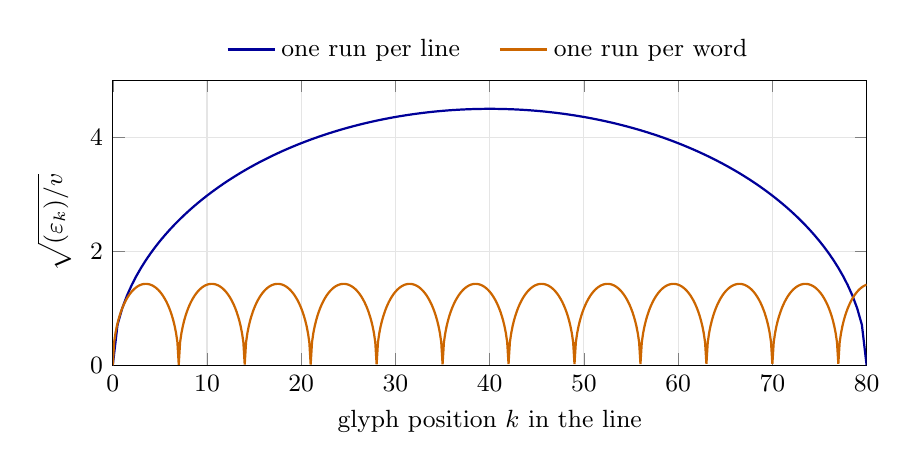
\begin{tikzpicture}
\begin{axis}[
  width=0.92\linewidth, height=5.2cm,
  xlabel={glyph position $k$ in the line}, ylabel={$\sqrt{\Var(\varepsilon_k)/v}$},
  xmin=0, xmax=80, ymin=0, ymax=5,
  legend style={at={(0.5,1.03)}, anchor=south, legend columns=2, draw=none, font=\small, /tikz/every even column/.append style={column sep=1.2em}},
  grid=major, grid style={gray!20}, tick label style={font=\small}, label style={font=\small}]
  \addplot[blue!60!black, thick, domain=0:80, samples=161] {sqrt(x*(80-x)/79)};
  \addlegendentry{one run per line}
  \addplot[orange!80!black, thick, domain=0:80, samples=561] {sqrt(mod(x,7)*(7-mod(x,7))/6)};
  \addlegendentry{one run per word}
\end{axis}
\end{tikzpicture}
\caption{Standard deviation of the selection error along a line of $80$ glyphs,
from \cref{eq:bridge}, for a single stretched run and for per-word runs with
words of six letters and a space. The per-word error returns to zero at every
word.}
\label{fig:drift}
\end{figure}
